\documentclass[a4paper]{jpconf}
\usepackage{graphicx}
\begin{document}
\title{The CMS Data Aggregation System}

\author{Valentin Kuznetsov}
\address{Cornell University, Ithaca, New York, USA}
\ead{vkuznet@gmail.com}

\author{Dave Evans}
\address{Fermilab, Batavia, Illinois, USA}
\ead{evansde@fnal.gov}

\author{Simon Metson}
\address{Bristol University, Bristol, UK}
\ead{s.metson@bristol.ac.uk}


%In a large modern enterprise, information is almost inevitably distributed among several database management systems. Despite considerable attention from the research community, relatively few commercial systems have attempted to address this issue. This article describes the technology that enables clients of IBM's federated database engine to access and integrate the data and specialized computational capabilities of a wide range of relational and non­relational data sources.

\begin{abstract}
%A meta-data plays significant role in a large modern enterprises, research experiments,
%digital libraries where it comes from different sources and distributed in a 
%variety of forms and digital formats. It is organized and managed by constantly
%evolving software using both relational and non-relational data sources. There is
%a big demand to enable information discovery from multiple sources.
%Here we discuss a new data aggregation system which consume and deliver information 
%from different relational and non-relational data sources on a concrete example 
%of large scale, distributed system of CMS physics experiment at LHC.

Meta-data plays significant role in a large modern enterprises, 
research experiments and digital libraries where it comes from different 
sources and distributed in a variety of forms and digital formats. 
It is organized and managed by constantly evolving software using 
both relational and non-relational data sources. Even though we can apply
information retrieval approach to non-relation data sources,
we can't do so for relational ones, where information can be accessed via
pre-established set of data-services.
%Even though we can access it via set of data-services, twikies, blogs, etc.,
%the information discovery across them is still a manual task.
% which prevent
%information discovery
%there is no coherent way for information discovery from different sources
%in heterogeneous, distributed environment with different security policies enforced.

Here we discuss a new data aggregation system which consumes, 
indexes and delivers information from different relational and 
non-relational data sources to answer cross data-service queries 
and explore meta-data associated with petabytes of experimental data. 
We combine simplpicity of keyword-based search with precision of RDMS
under the new system. The aggregated information being collected from various sources,
allowing end-users to place dynamic queries, get precise answers and 
trigger information retrieval on demand. Such close to real-time system 
based on studies  of use cases of the CMS particle physics experiment at 
the LHC where we used a large scale, distributed computing system 
to motivate the work.

\end{abstract}

\newpage

\section{Introduction}
The European Organization for Nuclear Research, known as CERN, plays a leading
role in fundamental studies of physics. But it is also known as a place where
many innovations in the area of computer science were developed, e.g. World Wide Web.
Today, the Large Hadron Collider (LHC) at CERN is marking a new era of High Energy
Physics (HEP), promising to deliver a few PB of data each year. 
At this scale the ``information discovery'' within heterogeneous, distributed 
environment become a key ingredient of successful data analysis in HEP.
%scientists are facing with a new set of problems in an area of
%``information discovery'' within heterogeneous, distributed environment.
The data and associated meta-data are produced in variety of forms and digital formats.
They are stored and retrieved from relational and non-releational data-sources, such as 
RDMS systems, document oriented databases, blogs, twikies, file systems and
customized applications, etc. 
%Its access is restricted by broad variety of security 
%policies enforced by individual sites and community in general.
Working in such environment requires a lot of expertise and our users
(in this case physicists) are always looking for simple, intuitive and flexible
tool(s) to look-up their desired data. A well-known solutions, such as data-services
and search engines tighted to a specific data sources and end-users are left 
with a manual task to bookkeep and relatate information from them.

Here we present a work on Data Aggregation System (DAS) designed for
CMS High-Energy Experiment at LHC which provides
ability to query, search and aggregate information from different 
data-services and trigger information retrieval on demand.

The rest of this paper is organized as following. 
In section \ref{RelatedWork} we discuss related work in a domain of 
keyword search over relational data sources.
Section \ref{DataModel} describes CMS experiment and its data model. In section
\ref{DAS} we present architecture of the DAS system, including discussion of its
various components. Finally, our results are summarized in section \ref{Results}.

%As was pointed out in \cite{Arms} a mixed content and 
%mixed meta-data and meta-data consistency should be considered as a whole in design 
%of the system to successful information discovery. 

\section{Related Work\label{RelatedWork}}
Even though the idea of keyword queries over the relational database(s)
%querying relation databases via keyword based search
%algorithms 
is not knew it is still under discussion in computer science domain.
A few alternative solutions has been proposed to address this issue
in last several years. In \cite{DBXplorer} the conjunctive keyword queries,
i.e. retrieval of only documents that contain all query keywords, has
been discussed. It requires that all keywords are matched in a row from
single table or joined tables. While \cite{QueryAnswer} make a step forward
by considering information around matched values and presents customized answers to
end-users over the generated new database. Those and other works\footnote{
For more information about
keyword based search over relational databases we redirect users to reference in
\cite{DBXplorer, QueryAnswer}.} 
are based on some kind of the graph over the underlying database and
moreover use a generated database out of the pristine one.
The proximity of the results in those techniques 
are mostly confined to the text-based values stored in a database, since the
keyword based search with numerical values 
need the precise knowledge of the related entity in a schema. For example, typing
100 can lead to inappropriate matches, such as row ids, and in order to be
answered correctly it requires additional keyword, clarifying its context, 
which should be matched with particular
entity (table.column) in the underlying database.
Therefore such approaches cannot be used to answer the logical questions, such as  
{\it find me total number of files whose size more then 20 but less then 
100 taken from january to february of 2009} which can be easily accomplished
using SQL syntax. 

To address those limitations an attempt to build a simple, intuitive and 
flexible query language was introduced in \cite{DBS-QL}\footnote{A similar but less
sophisticated approach was done in \cite{AMI}}.
It represents a power of SQL while hiding underlying relational schema from 
the end-users. As a results a human questions were intuitively mapped into 
simple queries. For example, the question
{\it I'm looking for files who contain data taken on certain date and located at
particular site} was represented as simple as \cite{DBS-QL}
\begin{verbatim}
find file where date 2009-01-02 11:59 CET and site = T2
\end{verbatim}
This solution represents a common use cases within HEP community and provide
intuitive mapping between mental model of end-users and underlying database back-end.

At the same time the data aggregation is commonly addressed in the context of
federated databases, see for example \cite{FedDB}. It unifies data coming 
from different RDMS systems into federated DB where SQL queries can be placed to 
search desired data. Even though it would be interesting to apply technique 
discussed in \cite{DBS-QL} to a federated database it still requires 
an access to the underlying database schema. This obviously creates a problem
working in distributed heterogeneous environment where different security policies
are in place.

To avoid those limitations we decided to build a keyword-search based system around
existing data-services whose nature and access policies are defined by developers.
Keeping in mind that meta-data can come in different forms and data formats
we used a document-oriented database back-end with full support of query language.
The key ingredients were the setup of the mapping and analytics services which provide
necessary glue across existing API/notations and user queries. This approach 
allows us to perform the data aggregation across various data-services, achieve
precise answers using keyword-based queries
and organize information retrieval on demand.
%to store meta-data information 
%We wanted to expand this approach further and apply it 
%to handle cross data-service queries from broad variety 
%of relational and non-relational data-sources within 
%our distributed heterogeneous environment.

\section{CMS data model\label{DataModel}}
The CMS, Compact Muon Solenoid, \cite{CMS} 
is one of the two large general-purpose particle physics detectors built on 
the proton-proton Large Hadron Collider (LHC) at CERN in Switzerland and France. 
It is designed to explore the frontier of High Energy Physics and provide physicists
ability to look at conditions presented at early stage of our Universe.
More then 3000 physicists from 183 institutions reprepresenting almost 
38 countries are involved in the design, construction and maintenance of the experiment.

The CMS distributed computing and data model \cite{CMSDataModel} 
is designed to process
and efficiently manage a few PBs of data expected each year
in CMS operation at LHC. The computing resources provided by members of CMS
collaboration are geographically distributed, 
interconnected via high throughput networks and operated by means 
of Grid software. The model allows to cover broad variety of
hardware, mass and storage elements and configuration of the
clusters. To accomodate efficient data processing CMS uses
a multi-Tier distributed model, where specific tasks of data taking,
processing, archival and distribution are assigned to each tier based
on CMS data model. For example, the Tier-0 center at CERN is responsible
for archiving the data coming out from the detector, prompt first pass reconstruction
and data distribution to Tier-1 centers. The 7 Tier-1 centers
located in France, Germany, Ialy, Spain, Taiwan, United Kingdom and United States
keep a portion (copy) of the data delivered by Tier-0 for further processing.
They provide storage and CPU power for high priority analysis jobs.
The Tier-2 centers, located at more then 50 sites around the world,
are dedicated for user analysis tasks and production of simulated data.

A broad variety of data-services being designed and developed to
maintain detector and production operations, including detector
conditions databases, data location and bookkeeping services,
data transfer and job monitoring tasks. Even though majority of them
are located at CERN, it was never been a requirement in CMS computing
and data model. For instance, the production teams operated at Tier-1,2
centers set up local services for data bookkeeping and operational
tasks. Based on their resources the choice of database back-end was
up to the site managers. Therefore the CMS software were designed to support different
DB back-ends and provide tools for migrating data across them.

Once such conglomerate of data-services starts operating an obvious
question arise: how to find out desired information across multiple data-services
in our distributed environment? Even though individual data-services were designed
to answer specific questions about the data they serve, the ability to search and relate
information among them was always a tedious human task. The growing amount of information
and desire to make cross-service queries force us to design and develop new
Data Aggregation System.

\section{Data Aggregation System\label{DAS}}
The design of the DAS system was based on previous studies of CMS Data 
Bookkeeping System (DBS) \cite{DBS, DBS07}. We carefully analyzed user
requests and queries placed into the DBS, their patterns, frequencies and latency. 
As a result we created a data discovery service \cite{DD}. Originally it used MVC
architecture and later, being re-factored as pure presentation layer on top of 
the DBS Query Language (DBS-QL) \cite{DBS-QL} with support of dynamic queries against
DBS back-ends. The DBS-QL \cite{DBS-QL} syntax was based on SQL query language, where 
we took away relations and details on underlying schema from end-users. 
This was achieved by usaging Dijkstras shortest path algorithm 
to establish necessary table joins based on provided information in user queries and
knowledge of foreign key relationships from auto-loaded database schema.
The DBS-QL keys exposed to end-users were choosen based on a jargon used by
physicists. They're internally mapped into database entitites and attributes, 
e.g. the {\it run} DBS-QL key refers to run number attribute of run summary table.
A quick adoption and wide usage of DBS-QL gave us confidence in choosen approach 
and provide a basis for building DAS system.

As was pointed out in \cite{Arms} a mixed content and 
mixed meta-data and meta-data consistency should be considered as a whole in design 
of the system to successful information discovery. 
Starting from this ground we designed DAS system as an
additional layer on top of the existing data-services
within CMS computing infrastructure by imposing the following set of requirements:
\begin{itemize}
\item support of keyword based search queries with ability to use condition operators;
\item pluggable interface to existing and up-coming data-service APIs;
\item support heterogeneous software environment and distributed nature of the data-services;
\item preserve security policies of individual data-services;
%\item be flexible to adjust to dynamic nature of data-service APIs, 
%due to continuously changing detector and software environments;
\item retrieve data on demand and aggregate them if necessary across
multiple data-services;
\item be transparent to data-services implementations and their data formats;
%\item support legacy data-services, applications and APIs.
\end{itemize}
\begin{figure}[htb]
\centering
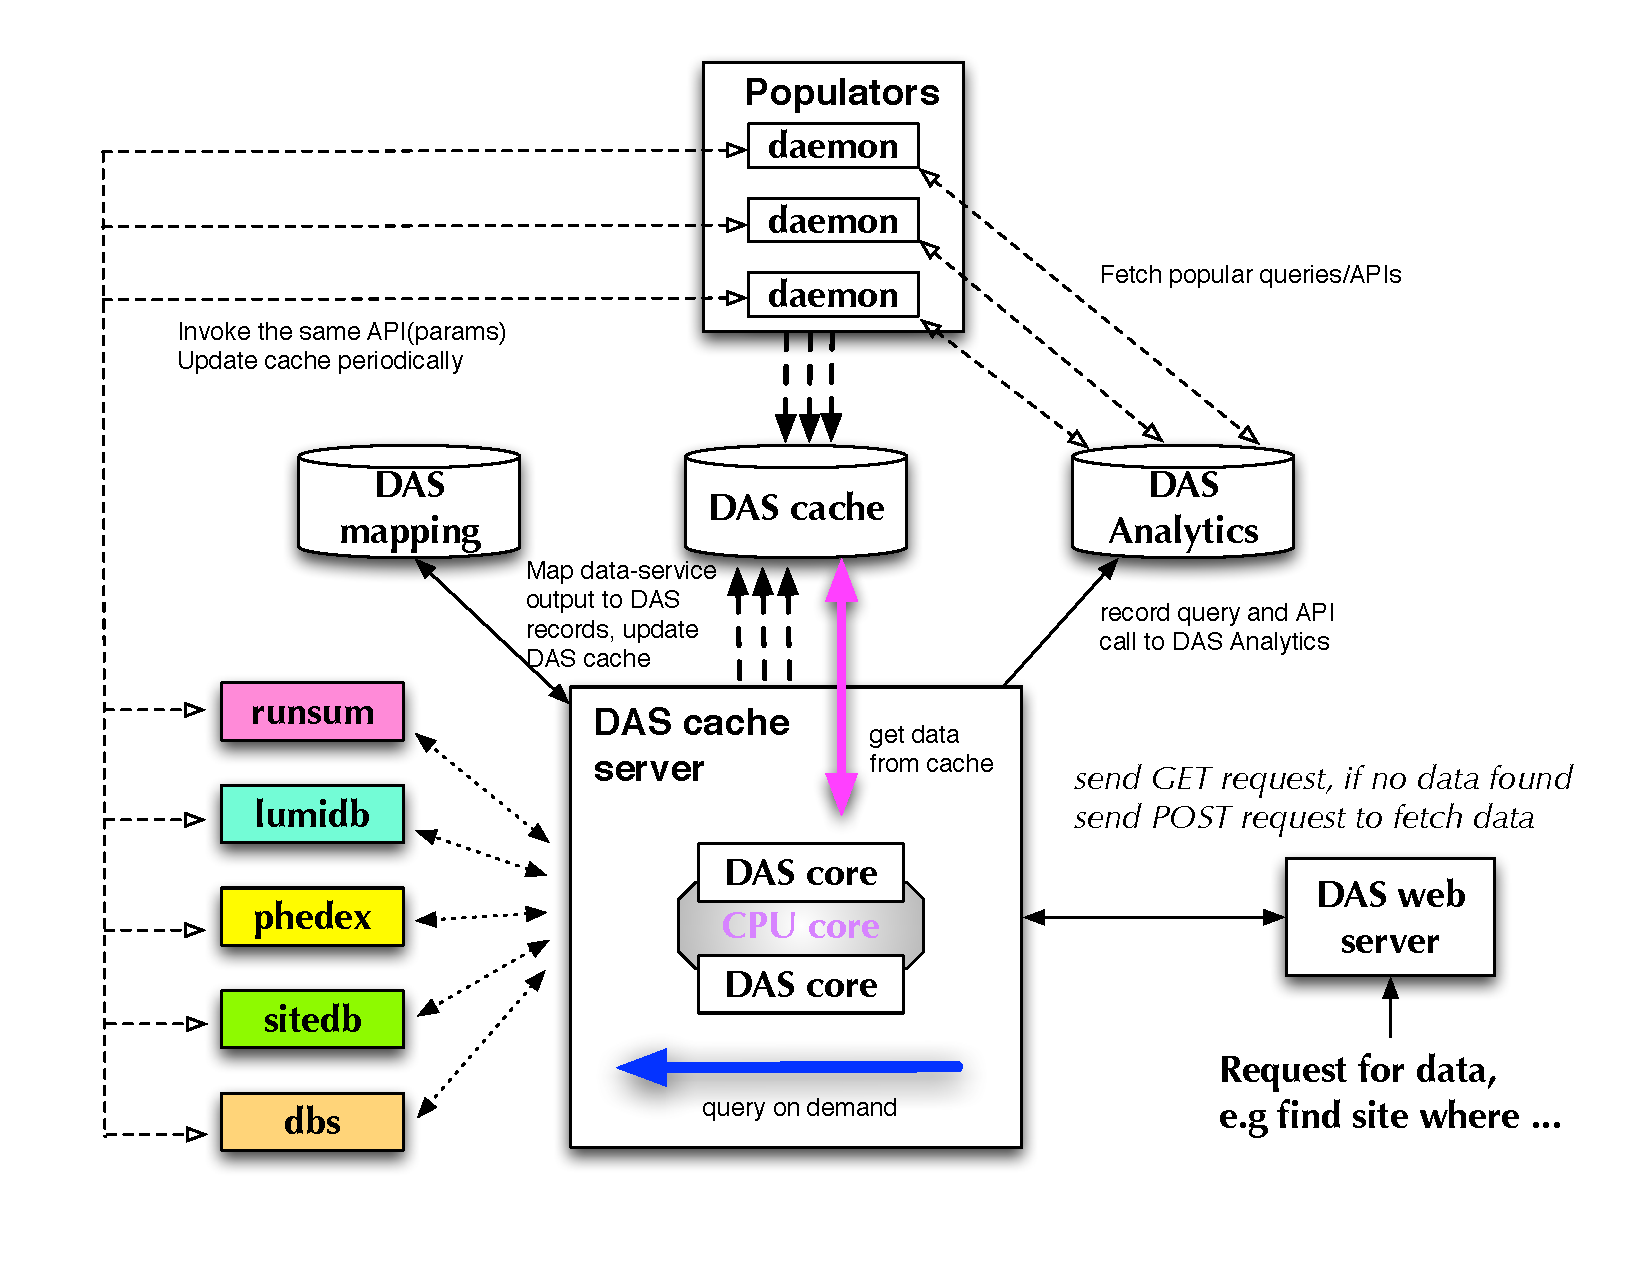
\includegraphics[width=150mm]{DAS_Cache_and_Analytics.pdf}
\caption{
The DAS architecture diagram. 
Input query where placed into analytics DB and mapped into set of
data-service APIs and their parameters. If superset of the query has been
found in DAS cache, the appropriate results were delivered back to users.
Otherwise a data-service APIs were invoked, triggering DAS cache population. 
Once data become available and aggregated in DAS cache users were able 
to see the results. This on demand system was supplemented by DAS robots 
(unix daemons) who were consulting DAS analytics database to enable data 
population into DAS cache for most common query requests.
}
\label{DAS_cache}
\end{figure}

\noindent
Due to this set of requirements, we rule out the choice of RDMS as DAS back-ends
for several reasons. We agreed to support dynamic queries, data
aggregation on demand and pluggable data-services. Therefore a choice 
of concrete schema for data storage was problematic. Moreover we didn't impose
any transactions and data persistency in DAS. This allows us to look 
for alternative IT solutions.
Through the analysis of available options, such as a file-based and memory caches, 
key-value databases, documented-oriented databases we made our choice in favor 
of the last technology. Among them we evaluated CouchDB \cite{CouchDB} and 
MongoDB \cite{MongoDB}. Both systems provide schema free document
storage, replication and fail-over features, but our choice in favor of 
MongoDB was obvious, due to its support of dynamic queries, 
full indexies, including inner objects and embedded arrays,
and auto-sharding. Our prelimiary benchmarks shown that it can sustain
the desired load and size for our meta-data information. We used 
document-oriented database, MongoDB, as a back-end for the three 
main DAS components: Mapping, Analytics and DAS cache databases, 
which will be discussed next. 

The DAS architecture is shown in Fig. \ref{DAS_cache}. It consists of the
following components:
core library with support of pluggable modules for data retrieval;
caching layer to store data-service output and aggregated results;
request service to handle user requests;
mapping DB to keep information about data-service APIs, their
notations and mapping to DAS;
analytics DB for query analysis and identification of pre-fetch 
strategies.

\subsection{DAS core}
The DAS core communicates with different data-services and retrieves
data on demand. This was done by invoking appropriate data-service plugin
upon the user request. Each plugin consists of DAS map,
data parser(s) suitable for data-service output format(s) into DAS common
data format (JSON) and was responsible for data-service API calls.
The data-service DAS map contains information about data-service APIs,
input and output parameters and their mapping to DAS keys. 
This information was stored into DAS Mapping DB which we discuss next.
Below you can see a typical DAS Mapping DB record for CMS
SiteDB data-service \cite{SiteDB}\footnote{We used regular expression 
patterns, evaluated during run time, to validate provided set of input 
paremters and DAS keys.}:
\begin{verbatim}
{"api": {"params": {"name": ""}, "name": "CMSNametoSE"}, 
 "api2das": [{"pattern": "re.compile('^T[0-3]_')", 
              "api_param": "name", 
              "das_key": "site"}], 
 "_id": "4ae1f8dfe2194e4581000014", 
 "system": "sitedb", 
 "daskeys": [{"pattern": "re.compile('^T[0-3]_')", 
              "key": "site", 
              "map": "site.name"}]}
\end{verbatim}
Although the majority of data-services looks alike
and their logic was abstracted, including parsers, there were a few
cases where special care was required. For instance,
we dealt with data-services which were only accessible via private network.
Therefore, a way to propagate user credentials was required, leading
to specific plugin implementation.

%All user queries were written to Analytics DB for further analysis, while
%mapping between data services were kept in Mapping DB. The data-service 
%output were re-mapped into DAS notations and, if necessary, aggregated 
%inside of the DAS cache.

\subsection{DAS Mapping DB}
DAS Mapping DB holded the mapping between data-service APIs and DAS keys exposed to
the users. It created a necessary glue between data-services and identifies
how their data can be related to each other. Basically Mapping DB was positioned 
as a {\it registration} service with ability to translate notations among data-services.
Upon identification of APIs which will participate in DAS activity 
we stored their names, input parameters, together with their type and accept 
values as regular expression patterns into the Mapping DB. 
Also we stored the mapping between data-service notations and DAS keys. 
For instance, the CMS DBS system \cite{DBS}
used {\it logical\_file\_name} notation to identify the name of the
logical file, while the same entity was called {\it lfn} in CMS PhEDEx system \cite{PhEDEx}.
Since both of them were referred to the logical file name, 
we map both notations into DAS key {\it file}.\footnote{We
also deal with physical file names, but still used {\it file} to refer to them in
DAS notations, since simple regular expressions were used to identify the
meaning of the {\it file} keyword from the provided value.}
Such keys, e.g. {\it file}, were exposed to the end-users as pre-defined keywords to
be used in search queries. For instance, end-users were able to type {\it file} in
order to get all file names known to DAS via data-services as well as
provide a concrete patterns associated with a file, e.g. {\it file=abc*}.
Under the hood, the appropriate data-service APIs were looked up along with appropriate
parameters to answer those questions. For example,
in aforementioned example, using {\it file} in DAS query cause call of DBS 
{\it listFiles} and PhEDEx {\it fileReplicas} APIs, respectively.
This approach gave power to end-users to express the meaning of their queries, especially
when they deal with numbers and achieve accuracy of results from DAS. 
For instance, users were able to type $run>10\,\,and\,\, run < 100$
to specify a range of run numbers to be looked up in DAS cache. At the same time
a full free text based keyword search is under development within MongoDB.

\subsection{DAS Analytics DB}
The DAS Analytics DB played a special role. It collected information
about user requests placed to the system. Each request was recorded. Upon its
decomposition into set of selection keys and conditions we also recorded
API name and input parameters into the Analytics database and 
keep updating their counter information for repeated calls. 
This allows to keep track of frequency of API calls and establish 
pre-fetch strategies for most common queries.

\subsection{DAS caching system}
The DAS caching system was used to store data-service results and aggregated
information in form of DAS records. As it shown in figure \ref{DAS_cache} 
the DAS cache server updates Analytics DB, requests and retrieve data from DAS cache
and aggregate data over there. The independent set of daemons, DAS robots, were
constantly monitor Analytics DB for most popular requests and pre-fetch most
common data into DAS cache.

Each user request placed to the system was parsed and set of selection
and condition keys were identified. They were mapped into set of
data service APIs and their input parameters. DAS
cache was checked for a queries with a similar set of selection and condition
keys used earlier.\footnote{Since DAS didn't hold
any data by default we cannot rely on data being present in a cache.
Moreover if we look-up data first, we cannot tell if it was complete
set or not, since earlier queries may retrieve only portion of the requested data.}
If the superset was found a data were
retrieved from the cache, otherwise a data-service APIs were
invoked and the results were collected and aggregated inside of DAS cache.

Apart from previous DBS-QL syntax we decided to drop its syntax and allow users
express their queries in a free text-based form. Such queries were transformed 
into MongoDB query syntax, who was used internally in
DAS core layer. It represents a set of selection keys and conditions as a JSON document.
For example, a query
{\it dataset site=T1\_CH\_CERN}
where transformed into 
{\it \{"fields" : ["dataset"], "spec" : \{"site" : "T1\_CH\_CERN"\}\}}.
Such syntax was perfect fit for us, since it allows to store all queries
as JSON documents into Analytics DB for further analysis. It is worthwhile to note that
MongoDB query syntax is very reach. It supports advanced queries with 
boolean expressions, conditional operators, regular expressions, etc. providing
a real power for our end-users.

\subsection{Data-services and aggregation}
As we outlined above the DAS Mapping DB becomes an authorative
source of information about all data-services participating in DAS.
Based on information stored in Mapping DB we were able to 
retrieve appropriate data from different data-services, re-map them into 
DAS notations and aggregate them on demand. For instance, the Data 
Bookkeeping System (DBS) and data location system (PhEDEx)
provided information about CMS data files. In former case, DBS 
stored information about files and their relationship to other 
physics objects, such as run and luminosity, while PhEDEx kept
information about the file location, e.g. details about sites 
holding copy of the files. Upon a user request to find a file, 
we were able to identify appropriate set of DBS and PhEDEx APIs, 
retrieve data from them, re-format their output to DAS notations 
and store results into DAS cache performing aggregation of matched 
objects. For instance, since both data-services returns in their
output a file name we used as a common key during aggregation.
This merged results represented a set of DAS records. Each DAS
record contains a standard DAS header, which identify look-up time,
request url, input parameters and API method as well as response 
version, expiration time and checksum of the output. Usage of this 
information was valuable contribution in debugging process of
data-services themselves, e.g. identification of not-matched records, 
latency studies, etc. Here is an example of DAS record representing
aggregation information between two SiteDB APIs, {\it CMStoSAMName} 
and {\it CMStoSiteName}, with API results merged under the {\it site} key.
\begin{verbatim}
{"_id": "4ae1e7ffe2194e4243000003", 
 "site":[{"samname": "CERN-PROD", "name": "T1_CH_CERN"}, 
         {"sitename": "CERN", "name": "T1_CH_CERN"}], 
 "das": [{"qhash": ["ed2b73067794d443ed56756d9b94f7bc"], 
          "ctime": 0.95439004898071289, "expire": 1256362175.7692671, 
          "url": "https://cmsweb.cern.ch/sitedb/json/index/CMStoSAMName", 
          "timestamp": 1256318975.7692671, "system": ["sitedb"], 
          "api": ["CMStoSAMName"], "version": "", "selection_keys": []}, 
         {"qhash": ["ed2b73067794d443ed56756d9b94f7bc"], 
          "ctime": 1.2158100605010986, 
          "api": ["CMStoSiteName"], 
          "url": "https://cmsweb.cern.ch/sitedb/json/index/CMStoSiteName", 
          "timestamp": 1256318974.7774379, "system": ["sitedb"], 
          "expire": 1256362174.7774379, "version": "", "selection_keys": []}
        ]
}
\end{verbatim}

%We used RESTful model \cite{REST} for all DAS cache server APIs.
%It allows us to share core library and other components during development of 
%various DAS clients, e.g. CLI, web interface, robots, etc. and hides
%complexity of access to individual data-services and their security policies
%as well as proper organize caching solution.
%For instance, to access on-line Run Summary information we were forced to use
%Grid certificates. Instead of propagating user certificate to data-service
%the DAS cache server works as a proxy to this server and used host certficiate 
%to serve such requests on behalf of the users.

\section{Results\label{Results}}
DAS was deployed to work with the following CMS data-services:
\begin{itemize}
\item DBS \cite{DBS}, Data Bookkeeping System, which collect information
about CMS meta-data;
\item PhEDEx \cite{PhEDEx}, Physics Experiment Data Export project, which
provides the data placement and the file transfer system for the CMS experiment;
\item SiteDB \cite{SiteDB} which 
records the CMS resources at the site, the resources pledged for the 
future, and it keeps track of CMS personnel at each site, including the 
roles and duties they fulfill in the collaboration;
\item RunSummary DB \cite{RunSummary} which collects information about run and triggers
conditions during data-taking;
%\item LumiDB \cite{LumiDB} collects information about Luminosity conditions;
%\item DQ \cite{DQ}, Data Quality data-service which collects information
%about detector conditions during data taking;
%\item Overview \cite{Overview}, collects information about CMS
%transfer rate, etc.;
\item Dashboard \cite{Dashboard} which monitors data collected from the 
distributed computing systems of the CMS experiment and LHC virtual organization
in general.
\end{itemize}
Each data-service has its own scope, size and lifetime. For instance the data
in PhEDEx are transient due to constant migration of CMS data, 
the DBS system were divided into dozen of individual instances, 
who has been used by different production teams for various bookkeeping tasks.
Figure \ref{db_size} shows current size of meta-data from aforementioned data-services.
\begin{figure}[htb]
\centering
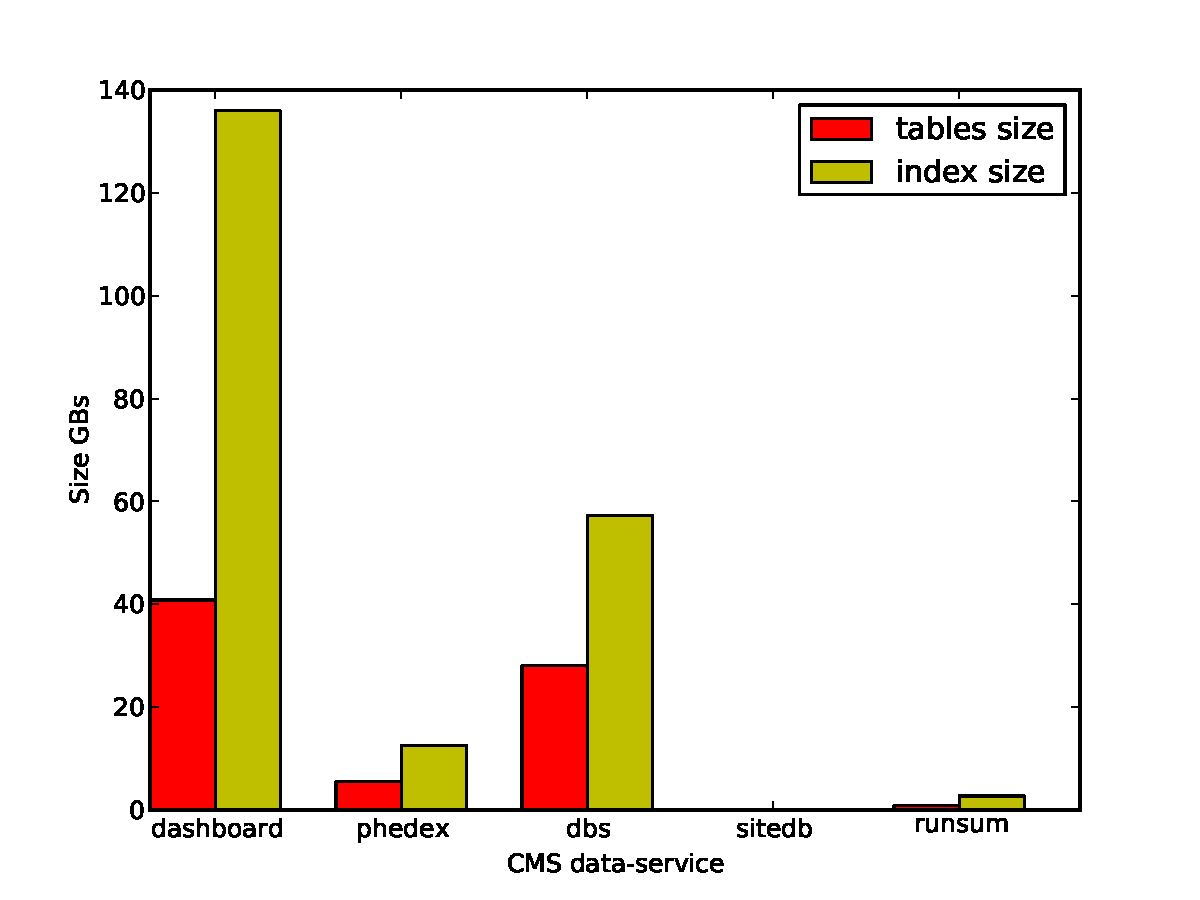
\includegraphics[width=100mm]{db_size.pdf}
\caption{
Current size of meta-data for CMS data-services participated in DAS, before
official data-taking. We anticipate to collect $\sim$500GB of meta-data
per year once LHC starts operating.
}
\label{db_size}
\end{figure}
%Typical
%size of individual DBS instance was around of fwe GBs, with overall DBS size of
%around of 50 GBs.\footnote{This include table and index sizes.}

At the moment we don't have exact numbers for amount of data which will stored to DAS,
but based on test performed during 
Cosmic Run at Full Tesla (CRAFT) data taking \cite{CRAFT09}
exercise we produced 0.3PB of data which
translate into $\sim50$ GB of meta-data stored in DBS system. Therefore
we can anticipate to collect $\sim500$GB of meta-data per year during data-taking period
at LHC.
%In CRAFT09 acquisition era, Tier-0 produced a total of 6.03
%billion events, 330TB in 32 datasets:
%AlCa/Calibration RAW: 926 million events, 29TB
%Physics RAW: 1.24 billion events, 147TB
%PromptReco: 1.24 billion events, 111TB
%Bulk ALCARECO: 2.34 billion events, 11TB
%Express FEVT: 105 million events, 24TB
%Express ALCARECO: 153 million events, 0.99TB
%HLTMON FEVTHLTALL: 31 million events, 7.4TB
%Above event numbers have signicant overlap by design, 
%2.2 billion unique events, including 524 million cosmic muon
%triggers
% 0.3PB - 50GB meta-data in DBS
% 3PB/y - x GB

Preliminary results of DAS performance are shown in Table \ref{DAS_benchmark}.
We benchmark time required to collect and aggregate block object information
from DBS and PhEDEx CMS data-services.

\begin{table*}[hbt]
\centering
\begin{tabular}{llllll}\hline
\hline

System & Format & Size & Records & Elapsed time & Elapsed time \\
& & & & no cached data & w/ cached data \\
\hline
DAS (DBS) & XML & 187MB & 368716 & 53 sec & 0.92 sec \\
DAS (PhEDEx) & XML & 164MB & 175884/170131 & 160 sec & 0.94 sec \\
DAS (aggregate) & JSON & 357MB & 374468 & 256 sec & 44.8 sec \\
\hline
\hline
\end{tabular}
\caption{Time required to fetch, parse and aggregate block information
from DBS and PhEDEx systems via their APIs. In the case of PhEDEx
system we show total number of fetched records 175884 together with
number of records merged in DAS 170131. The total number of DAS records 
were calculated as number of aggregated records plus left over, non-matched records,
from both systems.}
\label{DAS_benchmark}
\end{table*}

Elapsed time measured during this test consist of the following componenets:
\begin{itemize}
\item[]
{\it
Elapsed time = retrieval time + parsing time + re-mapping time 
        + cache insertion/indexing time 
        + (aggregation time) + (output creation time)
}
\end{itemize}
Here the {\it retrieval time} is a time required to access data from remote data-service,
{\it parsing time} is a time required to read and parse received data, {\it re-mapping time}
is a time to convert notations used by data-service to DAS ones for every object
we parse, {\it cache insertion} and {\it indexing time} represents time spend to add objects into
the DAS cache, {\it aggregation time} is required to merge objects into DAS records based
on their common key (block name in this case) and {\it output creation time}
is a time required to write DAS records to disk. Please note that last two
components, {\it aggregation} and {\it output creation time}, were only applied to
final DAS step and not to time spent in individual data-services.

%DAS execution time (phedex) 160.606897116 sec
%DAS execution time (dbs) 52.5349619389 sec
%DAS execution time 256.0670228 sec, Sat, 28 Nov 2009 15:46:39 GMT
%
%DAS execution time (phedex) 0.952513933182 sec
%DAS execution time (dbs) 0.951184034348 sec
%DAS execution time 44.7982931137 sec, Sat, 28 Nov 2009 15:52:11 GMT

The individual DAS components (DBS and PhEDEx) shown roughly the same performance.
Although the time of PhEDEx component was divided among: retrieval + parsing 
time $\sim$110 sec and merging step $\sim$50 sec.

As you can see from Table \ref{DAS_benchmark},
the time spent to read DAS records (last column) from the cache was quite
reasonable, roughly 1 second for both systems. While final time to
get DAS records on disk was about 45 seconds. This was mostly due to I/O and
conversion between binary data format used in database (BSON) to JSON.
All operations were performed on a single CPU core and obviously can be done
in parallel.

Based on this results we measured that we can achieve 7000 docs/sec rate
for insertion, 3400 docs/sec for aggregation and 8500 docs/sec for reading operation
in DAS, which is suitable for our 
needs.\footnote{We were satisfied with performance of the DAS prototype,
even though it throughput can be increased by few times
using C++ DB driver instead of python one used in this system.}

\section{Summary}
We presented new data aggregation service (DAS) developed for CMS High-Energy experiment
at LHC, CERN, Geneva, Switzerland. It was designed to provide caching and
aggregation layer on top of the existing relational and non-relation data-services
mostly in real time fashion. All the data were retrieved on demand basis,
while data pre-fetching of most common queries is in our plans. We developed
prototype in python for DAS system which is under commissioning phase right now 
and performed performance studies shown in this paper. 
The CMS experiment is started to
collect data from November 2009 and we expect to write about PB of data each
year to tape. In addition, the Monte-Carlo samples will be produced at this scale.
Based on test studies performed in CMS, we expect that total size of
meta-data produced by experiment each year will be of the order of
$\sim500$GB. The DAS should sustain such load and will provide generic 
``data-discovery'' service for CMS experiment in years to come.

\section{Acknowledgments}

This work was supported by the National Science Foundation and Department of Energy of the United States of America. Fermilab is operated by Fermi Research Alliance, LLC under Contract
No. DE-AC02-07CH11359 with the United States Department of Energy.

\section*{References}
\begin{thebibliography}{9}
\bibitem{DBXplorer}
Sanjay Agrawal, Surajit Chaudhuri, Gautam Das: DBXplorer: A System for
Keyword-Based Search over Relational Databases. ICDE 2002: 5-16

\bibitem{QueryAnswer}
Georgia Koutrika, Alkis Simitsis, Yannis E. Ioannidis: Pr\'{e}cis: The Essence of
a Query Answer. ICDE 2006: 69-78

\bibitem{DBS-QL} V. Kuznetsov, D. Riley, A. Afaq, V. Sekhri, Y. Guo, L. Lueking,
``The CMS DBS Query Language'', CHEP 2009

\bibitem{AMI}
Altas AMI web portal:
http://ami.in2p3.fr/opencms/opencms/AMI/www/Tutorial/AMIMediation.html

\bibitem{FedDB}
L. Haas, E. Lin,
``IBM Federated Database Technology'', \\
http://www.ibm.com/developerworks/data/library/techarticle/0203haas/0203haas.html

\bibitem{CMS} CMS Collaboration R. Adolphi et al., The CMS experiment at the CERN LHC, JINST, 0803, S08004 (2008)

\bibitem{CMSDataModel} 
.Grandi, D.Stickland, L.Taylor et al., The CMS Computing Model, CERN-LHCC-2004- 035/G-083 (2004);
A. Fanfani et. al.,
``Distributed Analysis in CMS'', to be published in Journal of Grid Computing.

\bibitem{DBS} A. Afaq, et. al. ``The CMS Dataset Bookkeeping Service'', CHEP 2007 
J.Phys.Conf.Ser, 119, 072001 (2008)

\bibitem{DBS07} A. Dolgert, V. Kuznetsov, C. Jones, D. Riley, 
``A multi-dimensional view on information retrieval of CMS data'', CHEP 2007

\bibitem{DD} https://cmsweb.cern.ch/dbs\_discovery

\bibitem{Arms}
C. R. Arms, W. Y. Arms, ``Mixed Content and Mixed Metadata 
Information Discovery in a Messy World'',
chapter from ``Metadata in Practice'', ALA Editions, 2004

\bibitem{MySQL}
http://www.mysql.com/

\bibitem{CouchDB}
http://couchdb.apache.org/

\bibitem{MongoDB}
http://www.mongodb.org/

\bibitem{REST}
Fielding, Roy Thomas ``Architectural Styles and the Design of 
Network-based Software Architectures'', Doctoral dissertation, 2000,
University of California, Irvine

\bibitem{PhEDEx}
Rehn et. al.,
``PhEDEx high-throughput data transfer management system'', CHEP06, Mumbai, India.
R. Egeland et al., Data transfer infrastructure for CMS data taking, Proceedings of Science,
PoS(ACAT08)033 (2008) ;
L. Tuura et al., Scaling CMS data transfer system for LHC start-up, J.Phys.Conf.Ser, 119, 072030 (2008)

\bibitem{RunSummary}
https://cmswbm.web.cern.ch/cmswbm/cmsdb/servlet/RunSummary

\bibitem{SiteDB}
https://cmsweb.cern.ch/sitedb/

%\bibitem{LumiDB}
%https://twiki.cern.ch/twiki/bin/view/CMS/CMS-DMWM-DBS-Luminosity

%\bibitem{DQ}
%Data-Quality DB reference

%\bibitem{Overview}
%https://cmsweb.cern.ch/overview/

\bibitem{Dashboard}
J. Andreeva, et. al,
``Experiment Dashboard – The Monitoring System for the LHC Experiments'',
GMW’07, June 25, 2007, Monterey, California, USA.

\bibitem{CRAFT09}
https://twiki.cern.ch/twiki/bin/view/CMS/CRAFT09AnalysisInfo

\bibitem{DBSearch}
D. Konopnicki, O. Shmueli,
``Database-Inspired Search'', 
Proc. of the 31st VLDB Conference, 2005.
\end{thebibliography}

\end{document}


